\documentclass[russian, 10pt]{beamer}

\beamertemplatenavigationsymbolsempty

\usepackage[utf8]{inputenc}
\usepackage[russian]{babel}

\usepackage{textcomp}
\usepackage{bm}
\usepackage{caption}
\usepackage{subfig}
\usepackage{listings}
\usepackage{hyperref}
\usepackage{pgfplots}
\usepackage{tikz}
\usepackage{amsthm}
\usepackage{pgf,pgfarrows,pgfnodes}
\usepackage{amsmath}
\usepackage{amsfonts}
\usepackage{amssymb}
\usepackage{wrapfig}
\usepackage{indentfirst}
\usepackage{setspace}
\usepackage{graphicx}
\usepackage{textcomp}
\usepackage{array}


\DeclareMathOperator{\E}{\mathbb{E}}
\DeclareMathOperator{\D}{\mathbb{D}}
\DeclareMathOperator{\R}{\mathbb{R}}


\usepackage{graphicx}
\usepackage[linesnumbered]{algorithm2e}

\begin{document}

\begin{frame}
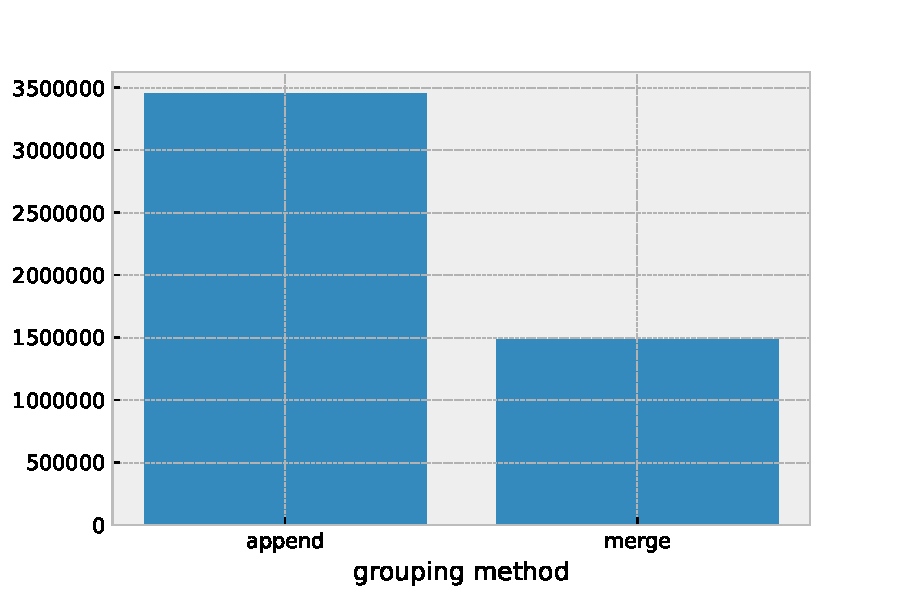
\includegraphics[scale=0.7]{images/grouping.pdf}

Данные из нескольких источников объединим в одну выборку посредством слияния. Оставим только уникальные элементы с заполнением недостающей информации по дубликатам.
\end{frame}


\begin{frame}

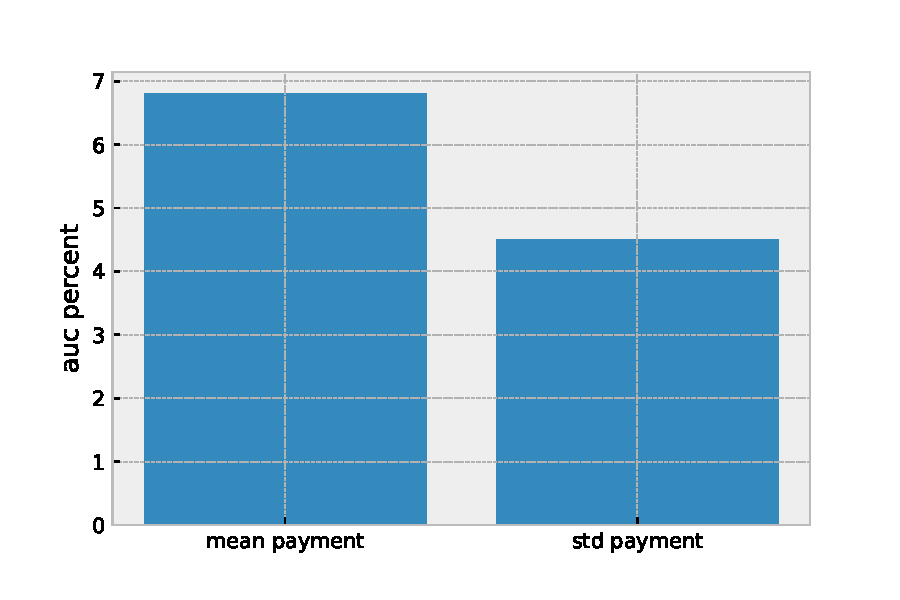
\includegraphics[scale=0.7]{images/meanstd_auc.pdf}

Признаки, вносящие значимый вклад в auc возьмём за основу. Около 0.56 и 0.54 для среднего и стандартного отклонения в признаке длины записи 'text payment discipline'.

\end{frame}

\begin{frame}

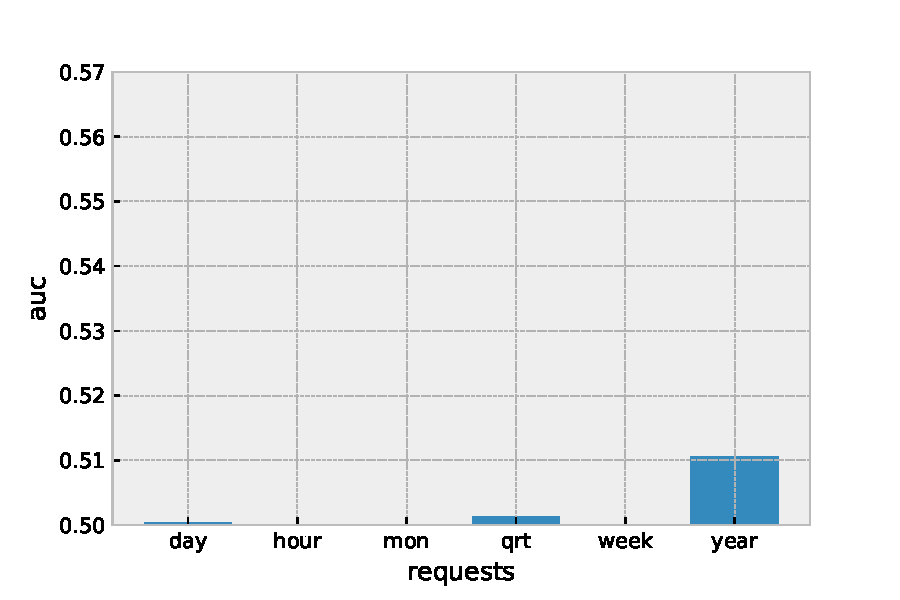
\includegraphics[scale=0.7]{images/requests.pdf}

Исследуем важность группы признаков -- количество запросов по временным промежуткам 'amt req *'. Значимым можно считать только признак 'amt req source year', на нём auc равен 0.51.

\end{frame}


\begin{frame}

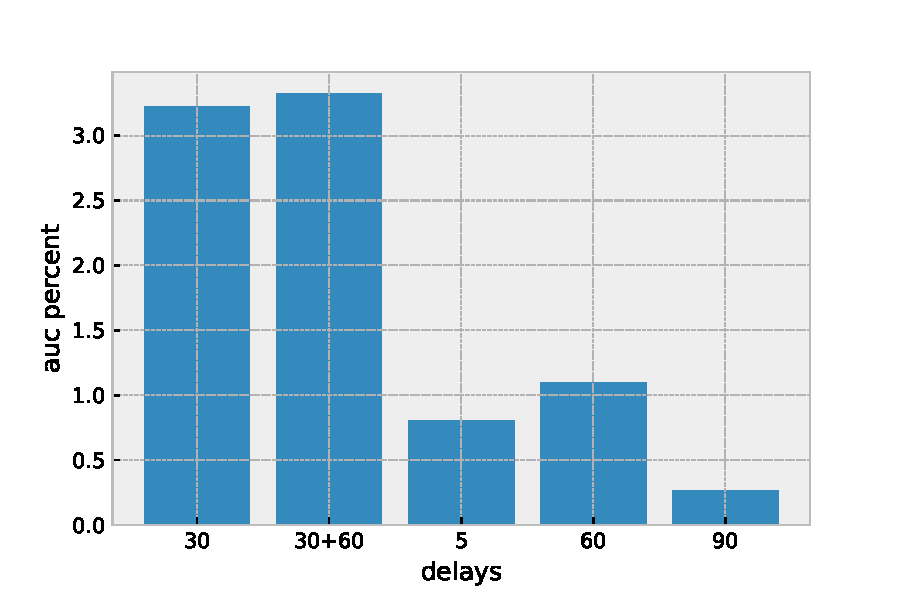
\includegraphics[scale=0.7]{images/delays.pdf}

Исследуем важность группы признаков -- число просроченных дней 'credit delay*'. Наиболее значимым является признак 'credit delay30' + 'credit delay60', на нём auc равен 0.53. Остальные группировки дают меньшее качество.

\end{frame}


\begin{frame}

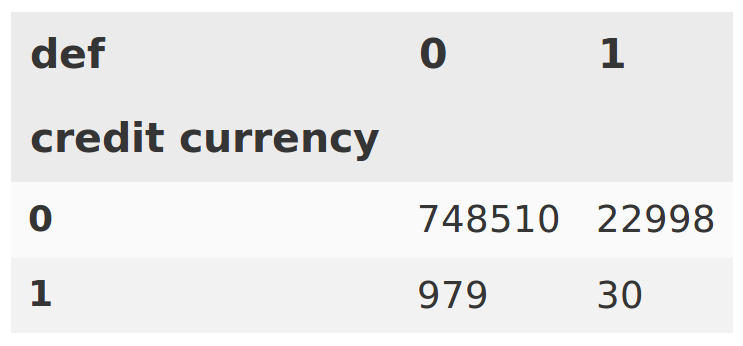
\includegraphics[scale=0.3]{images/currency.png}

\large
$AUC=0.50017$

Попарной упорядоченности между признаком валюты и целевым вектором нет.

\end{frame}


\begin{frame}


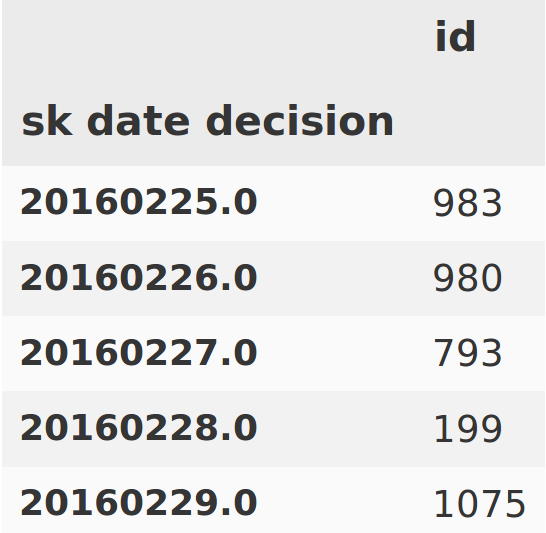
\includegraphics[scale=0.3]{images/sk_train.png}
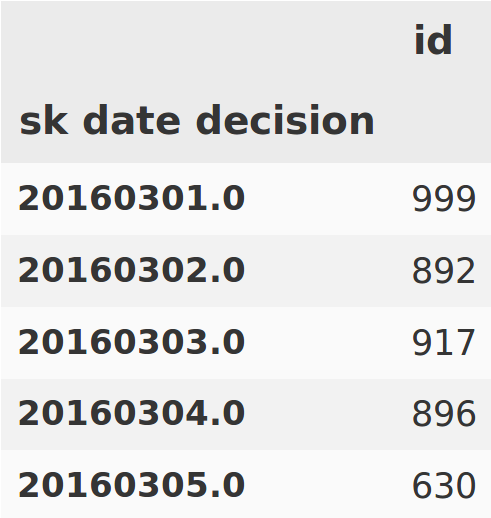
\includegraphics[scale=0.31]{images/sk_test.png}

Последние записи обучающей и первые записи контрольной выборок, упорядченных по номеру 'sk date decision'. Пересечения в выборках по данному признаку нет.
\end{frame}

\begin{frame}

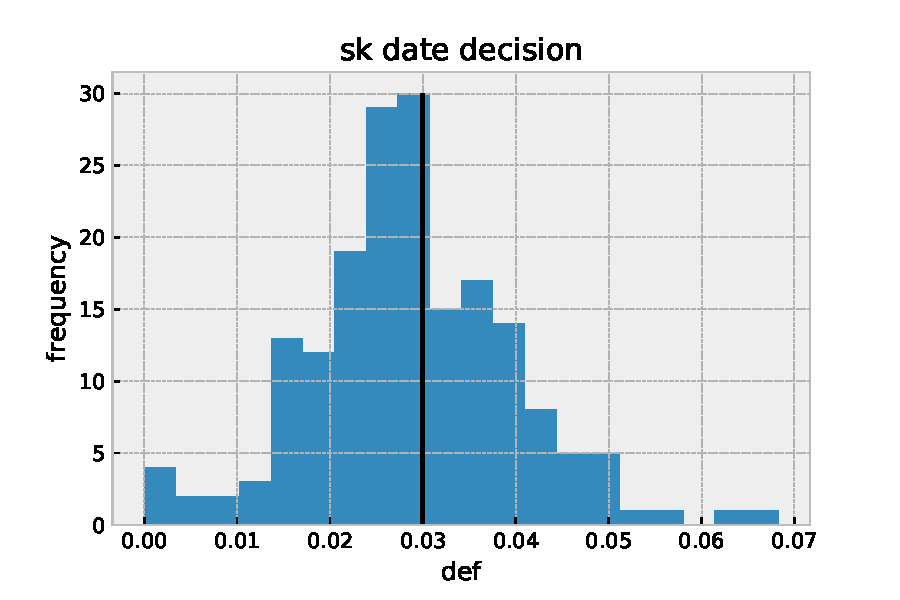
\includegraphics[scale=0.7]{images/sk_date_decision.pdf}

Однако распределение невыплаты по дате распределения заявки не вырождено и несёт в себе некоторую информацию. В этом должен быть смысл. На сайте конкурса об это признаке сказано отдельно.

\end{frame}


\end{document}